
\documentclass[xcolor=dvipsnames]{beamer}

\setbeamertemplate{navigation symbols}{}
% \setbeamertemplate{background}[grid][step=1cm]
\useoutertheme{infolines}
\usecolortheme[named=violet]{structure}
\setbeamertemplate{items}[circle]

\usepackage{tikz}
\usetikzlibrary{arrows,shapes,backgrounds}
\usepackage{listings}
\usepackage{graphicx}
\usepackage{color}
\usepackage{hyperref}
\usepackage{xspace}

\newcommand{\app}[1]{\textbf{\textit{#1}}\xspace}
\def\waf{\app{waf}}
\def\hwaf{\app{hwaf}}
\def\worch{\app{worch}}

\author[Brett Viren]{Brett Viren}
\institute[BNL]
{
  Physics Department
  
  
\includegraphics[height=1.5cm]{bnl-logo}
}
\title[LBNE Software Installation System]{LBNE Software Build and Configuration System}
\date[]{LBNE Collaboration Meeting 2013/09}


\begin{document}

\lstset{%
  emphstyle=\color{red},
  keywordstyle=\color{black}\bfseries,
  basicstyle=\footnotesize\ttfamily,
  identifierstyle=\color{DarkOrchid}\ttfamily,
  commentstyle=\color{Brown}\ttfamily,
  stringstyle=\color{blue}\ttfamily,
  showstringspaces=false}

\begin{frame}
  \titlepage
\end{frame}
\begin{frame}
  \frametitle{Outline}
  \tableofcontents    
\end{frame}

\section{Problems To Solve}

\begin{frame}
  \frametitle{LBNE Software Ecosystem}
  \small
  Where we are:
  \begin{itemize}
  \item No automated, cross platform, build system exists
  \item Distributed, multi-country collaboration, diverse expertise.
  \item So far, a largely Fermilab-centric mind-view towards software and computing.
  \item Existing LBNE software requires a \textbf{large} number of supporting packages, including leading-edge C++ compiler.
  \item Fermilab installation managed largely by one person\footnote{Thanks Lynn Garren!} with responsibilities to other experiments.
  \item We lack an overabundance of software expertise in the collaboration.
  \end{itemize}
  What we need:
  \begin{itemize}
  \item[$\rightarrow$] Control over the software and computing we rely on
  \item[$\rightarrow$] Get the existing software working at home institutions and laptops
  \item[$\rightarrow$] Facilitate further software development
  \end{itemize}
\end{frame}

\begin{frame}
  \frametitle{Note on role of UPS: current and desired dependencies}
  \begin{columns}
    \begin{column}{0.6\paperwidth}
      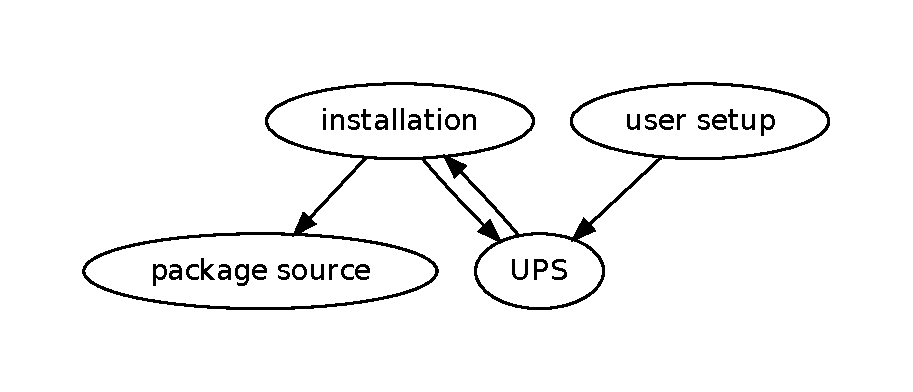
\includegraphics[width=\textwidth]{ups-deps}
    \end{column}
    \begin{column}{0.4\paperwidth}
      FNAL build system: UPS is required for both installation and
      usage.
    \end{column}
  \end{columns}
  \vspace{-5mm}
  \hrule
  \vspace{-5mm}
  \begin{columns}
    \begin{column}{0.5\paperwidth}
      Want: Installation system not dependent on UPS, allow
      alternative environment management systems. \\
      \vspace{1cm}
      {\footnotesize (arrows indicate direction of dependence)}
    \end{column}
    \begin{column}{0.4\paperwidth}
      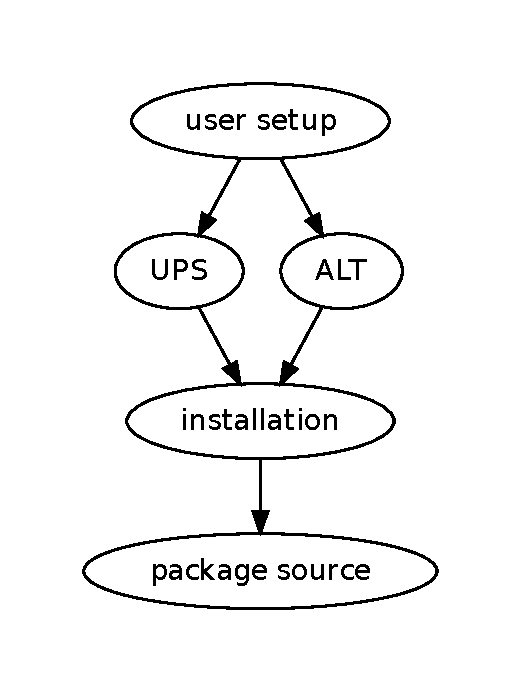
\includegraphics[width=\textwidth]{worch-deps}
    \end{column}
  \end{columns}
\end{frame}

\begin{frame}
  \frametitle{Current LBNE Suite}
  An incomplete (?) list of the packages making up LBNE software:
  \begin{description}
  \item[build tools] \texttt{cmake, gmp, ppl, mpfr, mpc, isl, cloog, gcc}
  \item[externals] \texttt{libxml2, sqlite, python, libsigcpp, libxml2, python, sqlite, tbb, xerces-c, lhapdf, mysql, postgresql, log4cpp, boost, fftw, cppunit, gccxml}
  \item[HEP] \texttt{root, geant4, cry, genie, pythia, globes} \\
    {\tiny (so far up through here)}
  \item[framework] \texttt{cpp0x, cetlib, fhicl-cpp, messagefacility, art, artdaq}(?)
  \item[LBNE] \texttt{larsoft, g4lbne}
  \end{description}
  Comprises, $\sim$20GB of build+install area \\
  (comparison: $2\mbox{-}3\times$ that for the Gaudi-based Daya Bay software).

  \vspace{5mm}
  
  Anything missing?
  \begin{itemize}
  \item I have nothing here for Near Detector!
  \end{itemize}
  
\end{frame}

\begin{frame}
  \frametitle{Strategy}
  Develop a (meta) build system which:
  \footnotesize
  \begin{itemize}
  \item Has a simple user interface driving an expert system.
  \item Captures all that is needed to install on all supported platforms in one location.
  \item Provides flexibility to install different suites or variations (debug vs. opt) and following different installation policies.
  \item Driven by LBNE needs but designed for general purpose use and comes with ``batteries included'' where practical.
  \item Maintains ``source code provenance'', use pristine, upstream source packages as input, but allow for application of any needed patches.
  \item Supports simple ``schema evolution'' of a the definition of the software suite,  easy incorporation of future suite upgrades, version controlled installation meta data.
  \item No hidden build failures, fail early, fail often.
  \item Makes use of multi-CPU installation machines.
  \item Based on community supported, Free Software tools.
  \end{itemize}
\end{frame}

\section{Overview of Installation System}

\begin{frame}
\tableofcontents[
currentsection,currentsubsection,
hideothersubsections,sectionstyle=show/shaded,
] 
\end{frame}

\begin{frame}
  \frametitle{Desires for the build system}
  What I really want is to be able to say to you:

  ``To use the LBNE build system all you must do is:''
  \vspace{5mm}
  \begin{enumerate}
  \item Download ``\textbf{it}''
  \item Run ``\textbf{it}''
  \item ???
  \item Profit.
  \end{enumerate}

  \vspace{5mm}

  Due to the large size of the LBNE software suite, the ``???''
  entails a few hours of you going and doing something else while the
  gears churn.
  
\end{frame}

\begin{frame}
  \frametitle{\textit{What is ``\textbf{it}''?}}
  ``It'' is called: ``\worch''.

  \vspace{4mm}
  \textit{What?  What the heck is that?}
  \begin{center}
    \textcolor{blue}{\worch = \textbf{w}af + \textbf{orch}estration}
  \end{center}

  \textit{You are loosing me!}

  \begin{itemize}
  \item This horrid name was the working title which just stuck.
  \item It ``orchestrates'' building a suite of software by
    interpreting a configuration file into \waf tasks and calling \waf
    for the heavy lifting.
  \end{itemize}
  From the \worch github page\footnote{\url{https://github.com/brettviren/worch}}:
  \begin{center}
    ``\textcolor{blue}{\textit{Let the orchestration \waf through the suite.}}''
  \end{center}
  \textit{Okay, that's cheesy.  So, what the heck is \waf?....}
\end{frame}

\begin{frame}[fragile]
  \frametitle{What is \waf?}

  \waf\footnote{\url{http://code.google.com/p/waf/}}:
  \begin{itemize}
  \item is not an acronym, nor a name with any particular meaning
  \item is a Python-based (v2.3-v3.1) framework for building build systems
  \item can be used as a \texttt{make/autoconf/cmake} replacement or as a layer
    on top to orchestrate a variety of ``native'', per-package build systems
  \item provides a task scheduling and dependency engine
  \item packaged as a single, self-contained, downloaded Python executable
  \end{itemize}
\begin{verbatim}
$ wget http://waf.googlecode.com/files/waf-1.7.12
$ chmod +x waf-1.7.12
$ alias waf=$(pwd)/waf-1.7.12
$ waf --version
waf 1.7.12 (c4b82f4337ebdf5236e844791a9faa346770d6db)
$ waf --help
\end{verbatim}

\end{frame}

\begin{frame}
  \frametitle{Aside: Synergy with ATLAS}
  
  With perfect timing, \textbf{Maxim Potekhin} pointed me to \waf and \textbf{Sebastien Binet} of
  ATLAS at the exact moment that I was becoming frustrated with my
  hand--written attempt at a scheduling/dependency engine.
  
  \textbf{SB} is using \waf as the basis for a next-generation build system for the ATLAS experiment.  His work includes: 
  \begin{itemize}
  \item a command line user interface: \hwaf
  \item replacing CMT with \waf
  \item migrating Gaudi + LCGCMT (in process) ``\texttt{tdaq}'' subsystem (done)
  \item its use for bootstrapping/creating analysis packages,
  \item contributions to \worch itself.
  \end{itemize}

  \vspace{2mm}
  \footnotesize
  Note of caution for LBNE and Fermilab: 
  \begin{itemize}
  \item ATLAS investigated CMake to replace CMT, found it unsuitable
    after two months of effort.
  \item 
    I still support replacing SRT with CMake in LArSoft, but for
    large-scale meta-build systems we should take heed.
  \item 
    We should investigate \hwaf/\waf to see if would be a worthy basis
    for LBNE ``native'' package builds.
  \end{itemize}
\end{frame}

\section{Examples}

\begin{frame}
\tableofcontents[
currentsection,currentsubsection,
hideothersubsections,sectionstyle=show/shaded,
] 
\end{frame}

\begin{frame}[fragile]
  \frametitle{Example: getting \worch}

\begin{verbatim}
$ git clone https://github.com/brettviren/worch.git
$ cd worch/
\end{verbatim}

  \begin{itemize}
  \item   Repository includes a main \waf ``\texttt{wscript}'' file, the ``\texttt{orch}'' python module, various example configuration files and documentation (including this presentation).

  \item   Will investigate packaging \worch + \waf into a single file like \waf itself is.

  \end{itemize}

  Github is the primary repository due to collaboration with ATLAS and
  some personal intentions to use \worch in other
  experiments/contexts.
    \begin{itemize}
    \item A symmetric mirror in Fermilab Redmine is possible.
    \end{itemize}


\end{frame}

\begin{frame}[fragile]
  \frametitle{Example: installation of the ``simple'' example suite}
{\tiny
\begin{verbatim}
$ waf --out=tmp-simple --prefix=install-simple --orch-config=examples/simple/*.cfg  configure
Setting top to              : /data3/bv/w/worch 
Setting out to              : /data3/bv/w/worch/tmp-simple 
Orch configuration files    : "examples/simple/buildtools.cfg", "examples/simple/gnuprograms.cfg", "examples/simple/simple.cfg" 
Orch configure envs         : "", "cmake", "hello", "bc" 
'configure' finished successfully (0.057s)

$ waf
Waf: Entering directory `/data3/bv/w/worch/tmp-simple'
Supported features: "dumpenv", "prepare", "makemake", "patch", "tarball", "vcs", "cmake", "autoconf"
[ 1/18] cmake_seturl:  -> tmp-simple/urlfiles/cmake-2.8.8.url
[ 2/18] cmake_download: tmp-simple/urlfiles/cmake-2.8.8.url -> tmp-simple/downloads/cmake-2.8.8.tar.gz
[ 3/18] cmake_unpack: tmp-simple/downloads/cmake-2.8.8.tar.gz -> tmp-simple/sources/cmake-2.8.8/bootstrap
[ 4/18] cmake_prepare: tmp-simple/sources/cmake-2.8.8/bootstrap -> tmp-simple/builds/cmake-2.8.8-debug/cmake_install.cmake
[ 5/18] cmake_build: tmp-simple/builds/cmake-2.8.8-debug/cmake_install.cmake -> tmp-simple/builds/cmake-2.8.8-debug/bin/cmake
[ 6/18] cmake_install: tmp-simple/builds/cmake-2.8.8-debug/bin/cmake -> install-simple/cmake/2.8.8/debug/bin/cmake
[ 8/18] hello_seturl:  -> tmp-simple/urlfiles/hello-2.8.url
[ 8/18] bc_seturl:  -> tmp-simple/urlfiles/bc-1.06.url
[ 9/18] hello_download: tmp-simple/urlfiles/hello-2.8.url -> tmp-simple/downloads/hello-2.8.tar.gz
[10/18] bc_download: tmp-simple/urlfiles/bc-1.06.url -> tmp-simple/downloads/bc-1.06.tar.gz
[11/18] bc_unpack: tmp-simple/downloads/bc-1.06.tar.gz -> tmp-simple/sources/bc-1.06/configure
[12/18] hello_unpack: tmp-simple/downloads/hello-2.8.tar.gz -> tmp-simple/sources/hello-2.8/configure
[13/18] bc_prepare: tmp-simple/sources/bc-1.06/configure -> tmp-simple/builds/bc-1.06-debug/config.status
[14/18] bc_build: tmp-simple/builds/bc-1.06-debug/config.status -> tmp-simple/builds/bc-1.06-debug/bc/bc
[15/18] bc_install: tmp-simple/builds/bc-1.06-debug/bc/bc -> install-simple/bc/1.06/debug/bin/bc
[16/18] hello_prepare: tmp-simple/sources/hello-2.8/configure -> tmp-simple/builds/hello-2.8-debug/config.status
[17/18] hello_build: tmp-simple/builds/hello-2.8-debug/config.status -> tmp-simple/builds/hello-2.8-debug/src/hello
[18/18] hello_install: tmp-simple/builds/hello-2.8-debug/src/hello -> install-simple/hello/2.8/debug/bin/hello
Waf: Leaving directory `/data3/bv/w/worch/tmp-simple'
'build' finished successfully (4m5.157s)
\end{verbatim}
}
\end{frame}

\begin{frame}[fragile]
  \frametitle{Visualization}
  \begin{columns}
    \begin{column}{0.3\paperwidth}
      {\footnotesize
      The "simple" example suite.

        Of note:
      \begin{itemize}
      \item 3 packages
      \item 2 atomic build groups
      \item File-based deps
      \item Inter-step deps\\
        {\tiny artificial dep shown:\\
          \verb|bc_install| \
          $\rightarrow$ \verb|hello_prepare|}
      \end{itemize}
      {\tiny (Arrows indicate reverse-dependency, \\
        or processing flow).}

      To generate:

\begin{verbatim}
$ waf [...] configure
$ waf --dot=simple.dot
$ dot -Tpdf \
  -osimple.pdf simple.dot
\end{verbatim}
}
{\tiny \texttt{dot} is from \url{http://graphviz.org}}


    \end{column}
    \begin{column}{0.6\paperwidth}
      \vspace{-1cm}
      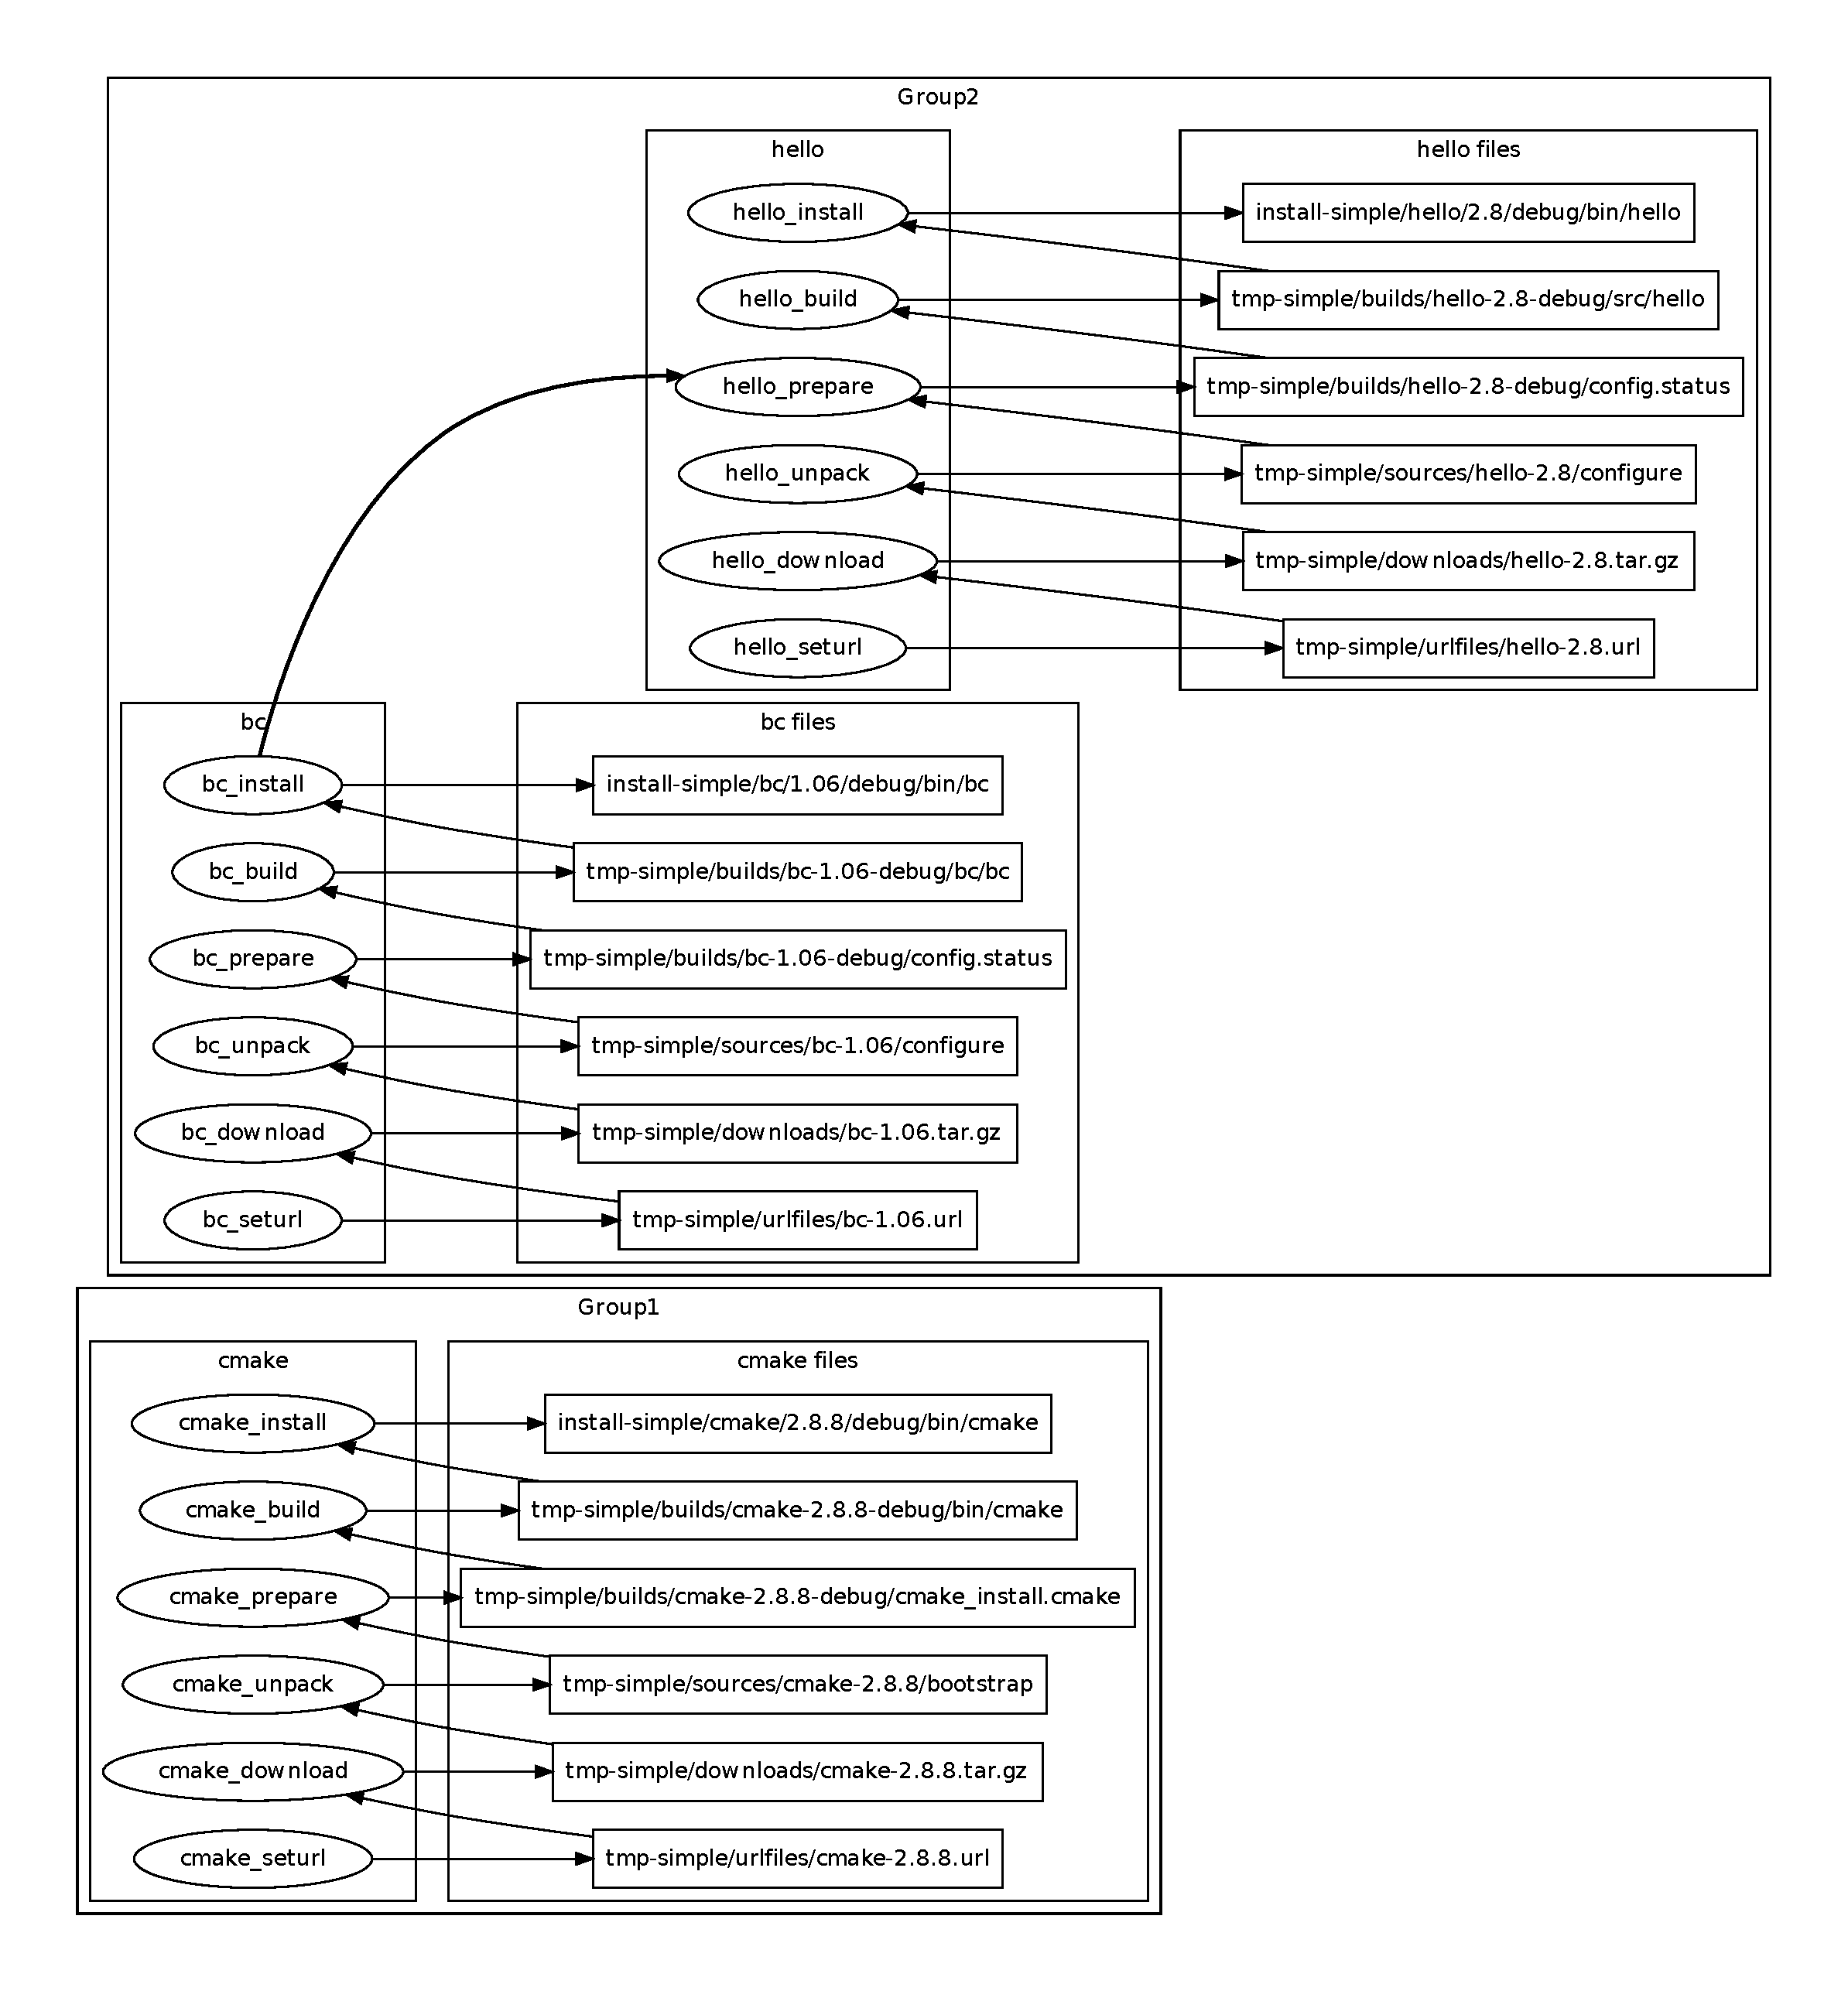
\includegraphics[height=\textheight]{simple}
    \end{column}
  \end{columns}

\end{frame}

\begin{frame}[fragile]
  \frametitle{Example: running \waf to build LBNE's suite }

  \footnotesize

  Read configuration file(s) and set installation destination:

\begin{verbatim}
$ waf --prefix=/path/to/install/area \
      --orch-config==examples/main/art.cfg configure
\end{verbatim}
  
  Build everything, with as many as 10 waf tasks at once:

\begin{verbatim}
$ waf -j10
\end{verbatim}

  Which shows:

\begin{verbatim}
[ 3/89] cmake_seturl:  -> tmp/urlfiles/cmake-2.8.8.url
[ 4/89] libxml2_seturl:  -> tmp/urlfiles/libxml2-2.8.0.url
[ 4/89] sqlite_seturl:  -> tmp/urlfiles/sqlite-3.7.17.url
[ 4/89] python_seturl:  -> tmp/urlfiles/python-2.7.3.url
[... etc for download, unpack, build, install ...]
[87/89] root_prepare: tmp/sources/root/CMakeLists.txt -> tmp/builds/root-5.34.09-debug/CMakeCache.txt
[88/89] root_build: tmp/builds/root-5.34.09-debug/CMakeCache.txt -> tmp/builds/root-5.34.09-debug/bin/root.exe
[89/89] root_install: tmp/builds/root-5.34.09-debug/bin/root.exe -> ../install/root/5.34.09/debug/bin/root.exe
'build' finished successfully (1h25m17.527s)
\end{verbatim}
  \begin{center}
      {\tiny (this build only went up through ROOT)}
  \end{center}
\end{frame}

\begin{frame}[fragile]
  \frametitle{Visualize the LBNE suite build}
  \begin{columns}
    \begin{column}{0.7\paperwidth}

      Three groups: \textit{buildtools, compiler} and \textit{externals} includes up through ``standard'' HEP packages:
      \vspace{5mm}

      \texttt{cmake, libxml2, sqlite, python, cmake, gmp, mpfr, mpc, isl, ppl, cloog, gcc, libsigcpp, tbb, xrootd, ROOT, Geant4, xercesc, log4cpp, mysql}.

      \vspace{5mm}
      In progress \textit{framework} and \textit{lbnesoft} groups with \texttt{cry, genie, globes, art, art\_externals, g4lbne, larsoft}.

      \begin{center}
        {\tiny (That things are too small to see is the point)}
      \end{center}
    \end{column}
    \begin{column}{0.225\paperwidth}
      \vspace{-10mm}
      \includegraphics[width=\textwidth]{pre-art}
    \end{column}
  \end{columns}
\end{frame}


\section{Configuration}

\begin{frame}
\tableofcontents[
currentsection,currentsubsection,
hideothersubsections,sectionstyle=show/shaded,
] 
\end{frame}

\begin{frame}
  \frametitle{Configuration} 

  If \worch ``orchestrates'' the install then its configuration file
  is the conductor's notes.  One mainly interacts with \worch through
  the configuration files in order to:
  \begin{itemize}
  \item Determine installation layout policy, Eg:
    \begin{itemize}
    \item match UPS ``product area'' conventions
    \item share/interleave different build options (\texttt{opt/debug}), platform labels
    \item build on fast local disk/ramfs, install to AFS/NFS
    \end{itemize}
  \item Specify list of packages to install
  \item Group them into atomically installed sets
  \item Define ``features'' implementing installation ``steps''
    \begin{description}
    \item [features] \textit{tarball, vcs, patch, autoconf, cmake, makemake}
    \item [steps] \texttt{seturl, download, unpack, patch, prepare, build, install}
    \end{description}
  \item Set parameters governing details of their build and installation
  \item Declare explicit inter-step dependencies
  \item Set package build and use environment variables
  \end{itemize}
\end{frame}

\begin{frame}[fragile]
  \frametitle{Basic configuration file syntax}

  Standard Python (\texttt{ConfigParser}) configuration file syntax \\
  (a.k.a. ``INI'' format).

  \begin{lstlisting}[language=bash,emph={section,section2}]
# this is a comment
[section]
key = value

[section2]
key = newvalue
key2 = value2
key3: equals-or-colons
  \end{lstlisting}

  Consists of a number of named \textbf{sections} containing a number
  of configuration \textbf{items} consisting of
  \textbf{key}/\textbf{value} pairs separated \\
  by ``\texttt{=}'' or ``\texttt{:}''.   Sections, keys and values are interpreted as strings.

\end{frame}

\begin{frame}[fragile]
  \frametitle{Extension: hierarchy of configuration parameters} 

  \begin{columns}
    \begin{column}{0.45\textwidth}
  \begin{lstlisting}[language=bash,emph={start,group,package,keytype},emphstyle=\color{red},emph={[2]group1,package1},emphstyle={[2]\color{blue}},emph={[3]groups,packages},emphstyle={[3]\color{magenta}}]
[start]
groups = group1, group2
key1 = val1
key2 = val2
key3 = val3

[group group1]
packages = package1, package2
key2 = grpval2

[package package1]
key1 = pkg1val1

[package package2]
key1 = pkg2val1

[keytype]
groups = group
packages = package
  \end{lstlisting}
    \end{column}
    \begin{column}{0.5\paperwidth}
      \small
      Hierarchy connected by section names
      \begin{itemize}
      \item Results in \textcolor{blue}{\texttt{package1}} having keys: 
        \begin{itemize}
        \item \texttt{key1 = pkg1val1}
        \item \texttt{key2 = grpval2}
        \item \texttt{key3 = val3}      
        \end{itemize}
      \item Likewise for \textcolor{blue}{\texttt{package2}} but with \\
        \texttt{key1 = pkg2val1}
      \item Special \textcolor{red}{\texttt{keytype}} section defines special variables to be
        interpreted as references to typed/named sections.
      \item Additional keytypes can be defined and parsed but \worch uses just \textcolor{magenta}{\texttt{groups}}
        and \textcolor{magenta}{\texttt{packages}}.
      \end{itemize}
    \end{column}
  \end{columns}

\end{frame}

\begin{frame}[fragile]
  \frametitle{Parameters in configuration}

  Configuration items form variables that can be referenced in other items.

  Reference a variable like ``\texttt{\{keyname\}}''.

  \begin{lstlisting}[language=bash,emph={package,version,gcc_version},emph={[2]PREFIX,tagsdashed},emphstyle={[2]\color{blue}}]
[start]
tags = debug
install_dir = {PREFIX}/{package}/{version}/{tagsdashed}
gcc_version = 4.8.1
groups = buildtools, compiler, externals
#...
[group compiler]
install_dir = {PREFIX}/gcc/{gcc_version}/{tagsdashed}
packages = gmp, ppl, mpfr, mpc, isl, cloog, gcc
#...
[package gcc]
version = {gcc_version}
#...
  \end{lstlisting}
  Variables are resolved late so ``flow down'' the hierarchy to take on meanings specific to each ``leaf'' keytype (\textcolor{red}{\texttt{package}} in this case).

  \textcolor{blue}{Some variables} and some other's default values are provided by \worch.
\end{frame}


\begin{frame}[fragile]
  \frametitle{Simple example - main file}
    \begin{lstlisting}[language=bash,emph={start,keytype}]
# worch/examples/simple/simple.cfg
[start]
groups = buildtools, gnuprograms
includes = buildtools.cfg, gnuprograms.cfg
group = gnuprograms
tags = debug
features = tarball autoconf makemake
download_dir = downloads
source_dir = sources
build_dir = builds/{package}-{version}-{tagsdashed}
install_dir = {PREFIX}/{package}/{version}/{tagsdashed}

[keytype]
groups = group
packages = package
    \end{lstlisting}
\end{frame}

\begin{frame}[fragile]
  \frametitle{Simple example - buildtools group file}
    \begin{lstlisting}[language=bash,emph={start,keytype}]
# worch/examples/simple/buildtools.cfg
[group buildtools]
packages = cmake
build_target = bin/{package}
install_target = bin/{package}

[package cmake]
version = 2.8.8
source_url = http://www.cmake.org/files/v{version_2digit}/{source_package}
unpacked_target = bootstrap
prepare_cmd = ../../{source_dir}/{source_unpacked}/bootstrap
prepare_cmd_options = --prefix={install_dir}
prepare_target = cmake_install.cmake
export_PATH = prepend:{install_dir}/bin
    \end{lstlisting}
\end{frame}

\begin{frame}[fragile]
  \frametitle{Simple example - gnuprograms group file}
    \begin{lstlisting}[language=bash,emph={start,keytype}]
# worch/examples/simple/gnuprograms.cfg
[group gnuprograms]
packages = hello, bc
source_url = http://ftp.gnu.org/gnu/{package}/{source_package}
environment = group:buildtools
unpacked_target = configure
prepare_target = config.status
build_target = bin/{package}
install_target = bin/{package}

[package hello]
version = 2.8
depends = prepare:bc_install

[package bc]
version = 1.06 
    \end{lstlisting}
\end{frame}

\section{Design}

\begin{frame}
\tableofcontents[
currentsection,currentsubsection,
hideothersubsections,sectionstyle=show/shaded,
] 
\end{frame}

\begin{frame}[fragile]
  \frametitle{Design Overview}
  \worch consists of these layers:
  \begin{description}
  \item[configuration] parses the configuration file into a dictionary
    of groups each consisting of a dictionaries of packages.
    Configuration items come from:
    \begin{itemize}
    \item configuration file(s) 
    \item hard-coded items required a package's \textit{features}
    \item a global set of required items
    \end{itemize}
  \item[features] each package has zero or more feature that map to a
    \worch Python method which produces one or more \waf tasks, based
    on configuration, to accomplish part of a package installation
    (eg: \texttt{tarball}, \texttt{autoconf}, \texttt{makemake}).
  \item[\texttt{wscript}] \waf uses \texttt{wscript} files (think
    \texttt{Makefile}) as entry points.  Normally \waf will use the
    single \texttt{worch/wscript} file but this will delegate if any
    \verb|worch/<package>/wscript| files exist.  So, if a building a
    package is too hairy to fit into existing \worch one can
    roll-your-own
  \end{description}
\end{frame}

\begin{frame}[fragile]
  \frametitle{Example: trivial \worch feature} 

  A feature is a method which constructs \waf tasks (task generators)
  based on its set of required configuration items.  Eg, from:

  \verb|worch/orch/features/feature_dumpenv.py|:
  \begin{lstlisting}[language=Python]
from .pfi import feature
@feature('dumpenv')
def feature_dumpenv(info):
    '''
    Dump the environment
    '''
    info.task('dumpenv', rule = "env | sort")
  \end{lstlisting}

  All modules like \verb|orch.features.feature_*| are auto-loaded by \worch.

  They declare tasks and inter-task (non-file) dependencies via the given \texttt{info} object.

  Some \verb|task()| options:
  \begin{description}
  \item[rule] specify the shell command to run or a Python function
  \item[source] specify a file (\waf Node) this task relies on
  \item[target] specify a file (\waf Node) this task produces
  \end{description}

\end{frame}

\begin{frame}[fragile]
  \frametitle{Example: a feature with requirements}
  \footnotesize

  \begin{itemize}
  \item Features provide list of required configuration items, with defaults

  \item ``Standard'' requirements are reused where appropriate.

  \item Requirements are available as data members or as format
    variables through the \texttt{info} object.

  \end{itemize}

  From: \verb|worch/orch/features/feature_autoconf.py|:
  \begin{lstlisting}[language=Python,basicstyle=\footnotesize\tiny,emph={requirements}]
requirements = {
    'unpacked_target': 'configure',
    'source_unpacked': None,
    'prepare_cmd': '../../{source_dir}/{source_unpacked}/configure',
    'prepare_cmd_options': '--prefix={install_dir}',
    'prepare_target': 'config.status',
    'build_dir': None,
}
@feature('autoconf', **requirements)
def feature_autoconf(info):
    def prepare_task(task):
        cmd = info.format("{prepare_cmd} {prepare_cmd_options}")
        return exec_command(task, cmd)
        
    info.task('prepare',
             rule = prepare_task,
             source = info.unpacked_target,
             target = info.prepare_target)
  \end{lstlisting}

\end{frame}

\begin{frame}[fragile]
  \frametitle{Dependencies}
  Tasks may depend on other tasks in a number of ways:
  \begin{description}
  \item[groups] All tasks of all packages in a group must finish before those of following groups begin.
  \item[files] The source/target files may form task dependencies
  \item[depends] explicit \texttt{depends} configuration items in the form of ``\verb|<step>:<otherpackage>_<otherstep>|'' make the current package's step depend on another package's step.
  \item[insertion] a feature may insert a step by name in front of another using names of the form \verb|<package>_<step>|.
  \end{description}
\end{frame}

\begin{frame}
  \frametitle{Steps}

  An open-ended but limited set of ``step'' names are used to provide
  common touchstones.  As more functionality is added to worch this
  set may enlarge.  New features should strive to reuse existing steps
  if they are conceptually compatible.
  \begin{description}
  \item[seturl] write the source archive into a file - this primes the dependencies based on files
  \item[download] download the source archive (tarball or VCS repository) given the URL
  \item[unpack] unpack the source archive (if tarball)
  \item[patch] apply a patch to an unpacked source archive
  \item[prepare] prepare the source for building (eg, autoconf, cmake)
  \item[build] build the package (eg, ``make'')
  \item[install] install the package (eg, ``make install'')
  \end{description}

\end{frame}

\section{Status and Future}

\begin{frame}
\tableofcontents[
currentsection,currentsubsection,
hideothersubsections,sectionstyle=show/shaded,
] 
\end{frame}

\begin{frame}
  \frametitle{Status}
  \begin{itemize}
  \item Basic functionality implemented and tested
  \item Configuration exists for simple examples and extensive
    LBNE-targeted groups: \textit{buildtools, compiler} and
    \textit{externals} (includes ``standard'' HEP packages)
  \item Initial target: Sci. Linux 6 (and somewhat Debian ``jessie'')
  \item Will continue to collaborate with ATLAS, exploit ``synergies''.
  \end{itemize}
\end{frame}

\begin{frame}
  \frametitle{Near Future}
  \begin{itemize}
  \item Finish incorporating art, LArSoft, genie, globes and g4lbne
  \item Get it into user's hands and fix any issues that uncovers.
  \item Target other popular platforms: SL5, Ubuntu and Mac OS X
    \begin{itemize}
    \item Set of supported platforms?
    \item Guided by recent survey.
    \item Every supported platform needs at least one responsible ``champion''.
    \end{itemize}
  \end{itemize}
\end{frame}

\begin{frame}
  \frametitle{Next-next Steps}
  \begin{itemize}
  \item Provide for user environment configuration
    \begin{itemize}
    \item produce UPS compatible configuration files and 
    \item develop independent environment management system
    \end{itemize}
  \item understand and satisfy Near Detector needs.
  \item Hooks into various LBNE software repositories
    \begin{itemize}
    \item continual integration, commits trigger rebuild,
      report failures
    \item likely use ``buildbot'', exploit existing experience at FNAL 
      \begin{itemize}
      \item [$\rightarrow$] want to run a buildbot on every supported platform.  Expect a cadre of ``platform champion'' to provide hardware and setup/maintenance effort.
      \end{itemize}
    \item learn of ``bad commits'' breaking the build ASAP.
    \item allow confidence when we upgrade (eg, new Geant4)
    \item run suite of validation jobs.
      \begin{itemize}
      \item[$\rightarrow$] detector/physics groups must develop these validation processes.
      \end{itemize}
    \end{itemize}
  \end{itemize}
\end{frame}

\end{document}